\section{Tracking Block Design}
\label{sec:tracking}

The tracking block uses camera inputs to calculate hand positions. Four modules
will comprise the block.

\begin{figure}
\centering
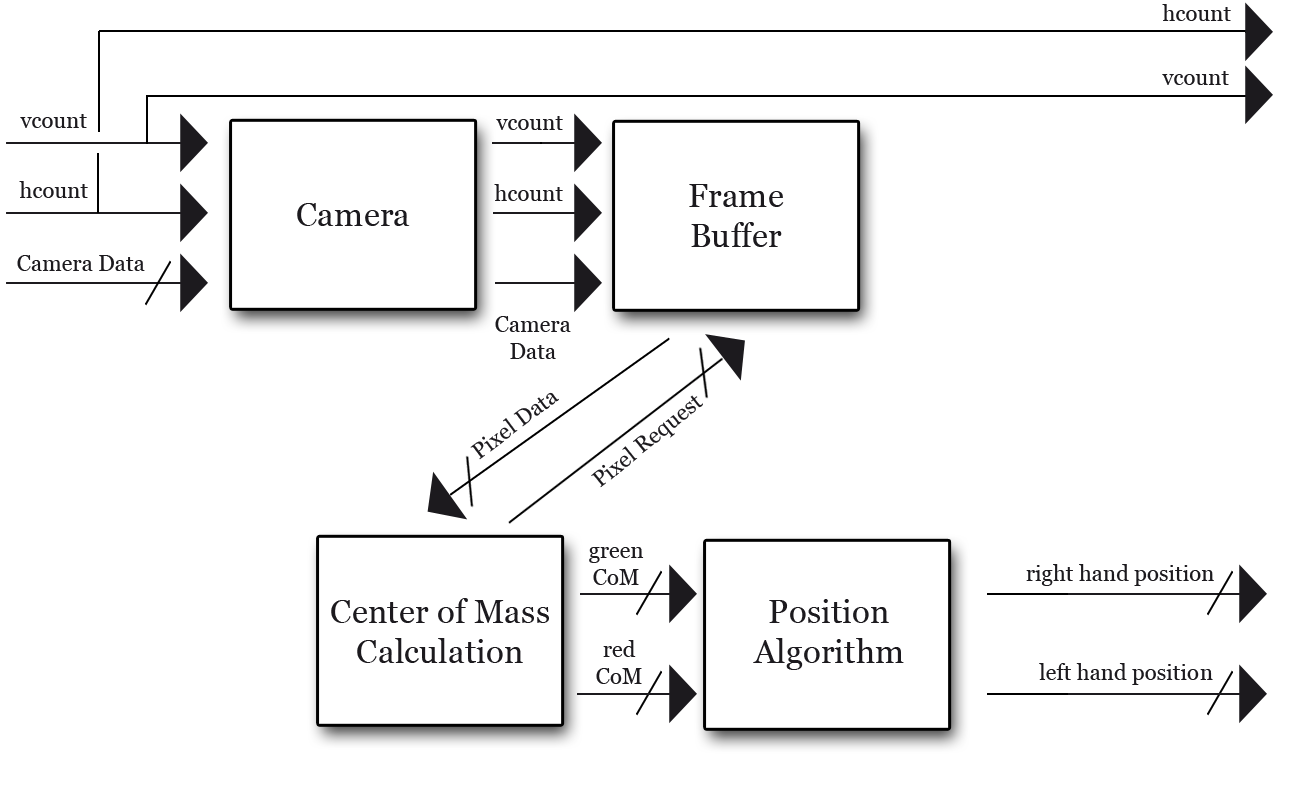
\includegraphics[scale=1]{img/tracking.png}
\caption{The tracking system has four primary steps. First information is
processed from the raw camera input. Second, frames are stored for later use.
Third, center of mass information is calculated for each color. Finally, a
smoothing function using past velocity and position information to prevent
errors. The result is accurate information describing the position of the
player's hands.}
\label{fig:tracking}
\end{figure}

\subsection{Camera Module}

The camera module will process inputs from the camera and down-sample them. The
basis for this module will be the already implemented 6.111 camera module
provided by the course staff. Modifications on top of this base will allow for
the functionality necessary for this game. Inputs will come directly from the
camera. Outputs will be control signals and pixel data.

\subsection{Frame Buffer}

A frame buffer will use ZBT memory to store two down-sampled frames from the
camera. It will take as input the control signals and pixel data from the camera
module and a number of bits from the downstream center of mass module specifying
which pixel to output next. It will output a single pixel of information and any
necessary control signals.

The complexity of this module is low, although it will use a significant amount
of ZBT memory and therefore require careful clock manipulation.

\subsection{Center of Mass Module}

The center of mass module calculates the center of mass of red, green, and blue
color in each frame fed from the camera. It takes as input pixel data and any
necessary control signals from the frame buffer and outputs the x and y
coordinates of the center of mass of each color.

This module is somewhat complex. It must do a weighted sum over all pixels on
screen. It will loop through all pixels on screen at 27 Mhz, storing in a set of
registers the running value of each center of mass. Division will be necessary
for the weighting calculation, significantly increasing the complexity of this
module. An approximation may be used that rounds all values to powers of two if
that is deemed accurate enough.

\subsection{Position Module}

The position module will take as input the center of mass information from the
center of mass module. It will output the position of each hand. This algorithm
will store the last position and velocity of each hand and use that information
to calculate the updated positions and velocities. This should allow for
improved accuracy when compared with a simply center of mass position
calculation.

This module will be fairly simple, using two registers to store past positions
and velocities, and running short algorithm to calculate a next position and
next velocity.

\subsection{Timeline}

This block will be the first goal for Turner Bohlen. Construction will proceed
in the order shown above, starting with the camera module and proceeding until
the position module is completed. A first working version of this block will be
completed before Thanksgiving.
